\documentclass[lmodern, utf8, seminar]{fer}
\usepackage{booktabs}
\usepackage{graphicx}
\usepackage{float}
\usepackage{listings}
\usepackage{color} %red, green, blue, yellow, cyan, magenta, black, white
\definecolor{mygreen}{RGB}{28,172,0} % color values Red, Green, Blue
\definecolor{mylilas}{RGB}{170,55,241}


\lstset{language=Matlab,%
    %basicstyle=\color{red},
    breaklines=true,%
    morekeywords={matlab2tikz},
    keywordstyle=\color{blue},%
    morekeywords=[2]{1}, keywordstyle=[2]{\color{black}},
    identifierstyle=\color{black},%
    stringstyle=\color{mylilas},
    commentstyle=\color{mygreen},%
    showstringspaces=false,%without this there will be a symbol in the places where there is a space
    numbers=left,%
    numberstyle={\tiny \color{black}},% size of the numbers
    numbersep=9pt, % this defines how far the numbers are from the text
    emph=[1]{for,end,break},emphstyle=[1]\color{red}, %some words to emphasise
    %emph=[2]{word1,word2}, emphstyle=[2]{style},    
}
\graphicspath{{images/}}

\begin{document}
\nocite{*}

\title{Automatska segmentacija lezije na MRI snimkama}

\author{Matija Marić}
\voditelj{prof. dr. dc. Igor Lacković}

\maketitle

\tableofcontents

\chapter{Uvod}

Segmentacija slika se bavi dekompozicijom slike u njezine sastavne dijelove (regije). Segmentirane regije imaju neka zajednička svojstva: uniformne su s obzirom na vrijednosti piksela ili imaju jednaku teksturu, imaju jasno definirane i jednostavne granice, zatvorene su i značajno se razlikuju od susjednih regija.
Najzastupljenija metoda segmentacije je detekcija rubova i metode zatvaranja tih rubova u granice regija.

Ovim radom istražiti će se metode detekcije regije lezija i tumora na medicinskim radiološkim snimkama na osnovi sličnosti značajki unutrašnjosti objekta, kombiniranje različitih snimki istih presjeka, određivanje rubova lezija na kombiniranim slikama i usporedba sa individualnim snimkama.

\chapter{Segmentacija bazirana na regijama}

Kod segmentacije bazirane na regijama umjesto da tražimo granice na osnovi diskontinuiteta poput rubova, regiju određujemo izravno na osnovi sličnosti značajki koji joj pripadaju.

\section{Metoda proširenja regije}

Metoda proširenja regije ({\it eng. region growing}) je postupak kod kojeg grupiramo piksele ili podregije u veće regije na osnovi kriterija pripadnosti istoj regiji (sličnost, susjednost, ...). Osnovni pristup je započeti sa početnim skupom točaka i širiti regiju postupno nadodajući sve susjedne točke koje imaju svojstva slična početnim točkama (npr. slične razine sive ili boje).

Odabir početnih točaka ovisan je o prirodi problema, ali u ovom radu će biti zadan ručno.

Jedan od problema je uvjet zaustavljanja. Proširenje regije treba prekinuti onda kad više ni jedan piksel ne zadovoljava uvjete pripadnosti regiji. Svojstva poput sivih razina, boje i teksture su lokalne prirode i ne uzimaju nužno u obzir značajke ostatka regije. Dodatni uvjeti koji mogu pomoći su prosječna siva razina proširene regije i sličnost sa početnim točkama ili oblik regije i veličina. Dodatni uvjeti vrijede naravno samo ako imamo model očekivanih rezultata.

Usporedbe sličnosti možemo raditi na osnovi sličnosti dvije susjedne točke, sličnosti okoline susjednih točaka ili sličnosti točke i centroide regije.

\begin{figure}[H]
	\centering
	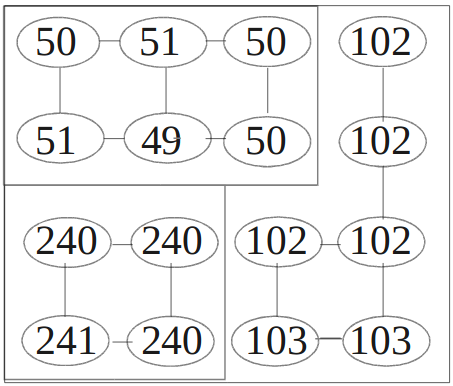
\includegraphics[width=0.6\textwidth]{similarity}
	\caption{Primjer gdje se točke smatraju sličnima ako je razlika vrijednosti manja od 5.}
	\label{fig:similarity}
\end{figure}

\section{Metoda dijeljenja i stapanja}

Kod metode dijeljenja i stapanja ({\it eng. split and merge}) sliku prikazujemo pomoću kvartartnog stabla ({\it eng. quad tree}). Počinjemo sa cijelom slikom segmentiranom u jednoj regiji, ako je regija neuniformna dijeli se na četiri dijela, ako su 4 susjedne regije uniformne onda se stapaju u jednu regiju.
Uniformnost možemo mjeriti pomoću razlike najveće i najmanje svjetline u regiji.

\begin{figure}[H]
	\centering
	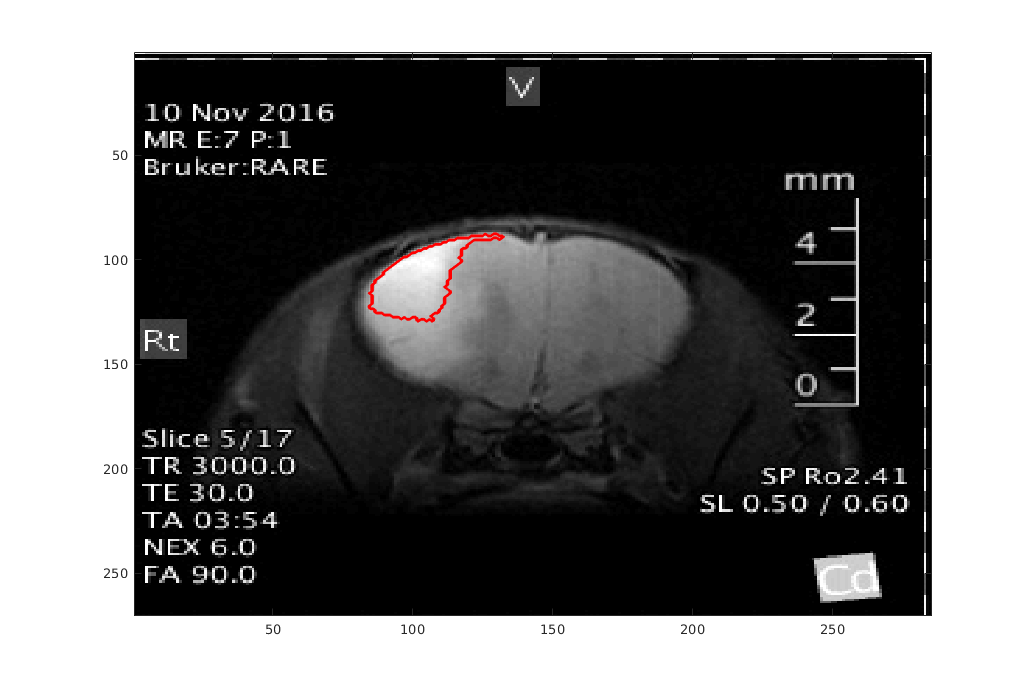
\includegraphics[width=0.7\textwidth]{regiongrow}
	\caption{Regija odvojena metodom proširenja regije sa parametrom maksimalne udaljenosti intenziteta $d = 0.15$}
	\label{fig:regiongrow}
\end{figure}

\chapter{Stapanje slika}

Postupak stapanja slika ({\it eng. image fusion}) je sakupljanje bitnih informacija iz više slika i kombiniranje u manji broj (obično jednu) slika. Stopljena slika je informativnija i preciznija od bilo koje pojedine slike i sadrži sve bitne informacije.

Kod stapanja slika cilj nije sažeti i smanjiti količinu podataka nego generirati prikladniju i jasniju sliku za interpretaciju i ljudima i algoritmima računalnog vida.
Ima široku primjenu u područjima gdje se koriste podaci višesenzorskih sustava poput satelitskih i medicinskih snimaka.

Metode stapanja slike se svrstavaju u dvije kategorije, stapanje u prostornoj domeni i u domeni transformacije. Neke od metoda u prostornoj domeni su Boveyeva metoda, PCA ({\it eng. principal component analysis}), IHS transformacija ({\it eng. Intensity-Hue-Saturation} prostor boja). Jedna važna metoda stapanja je tehnika bazirana na visokopropusnom filtriranju koja služi za izoštravanje slike tako da poveća doprinos visokofrekventnih značajki.

Nedostatak stapanja u prostornoj domeni je spektralna distorzija na stopljenoj slici koja može biti problem kod daljnje analize, npr. u problemu klasifikacije. Metode stapanja u frekvencijskoj domeni su bolje u otklanjanju distorzije.

\section{Stapanje slika wavelet transformacijom}

\subsection{Wavelet transformacija}
Waveleti su porodica funkcija valovitih oscilacija u kratkom intervalu, koje počinju sa nultom amplitudom i završavaju sa nulom. Konvolucijom možemo koristiti wavelet funkcije za analizu signala koji sadrže slične uzorke. Odgovarajući skupovi komplementarnih waveleta koji mogu rastaviti signal bez rupa i preklapanja su reverzibilni. Takve skupove možemo koristiti za kompresiju/dekompresiju sa minimalnim gubitkom. Primjer kompresijskog algoritma koji koristi diskretnu wavelet transformaciju je JPEG2000. Iste funkcije koristimo za dekompoziciju i kombiniranje slika u domeni transformacije. 

\begin{figure}[H]
	\centering
	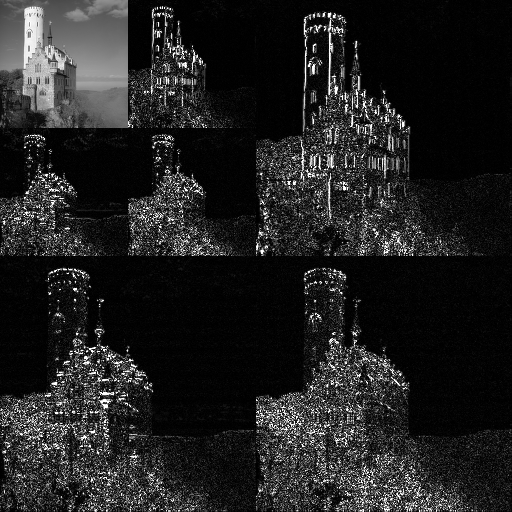
\includegraphics[width=0.6\textwidth]{jpeg2000}
	\caption{Primjer 2D diskretne wavelet transformacije koja se koristi u JPEG2000 kompresiji}
	\label{fig:jpeg2000}
\end{figure}

\subsection{Wavelet stapanje u MATLAB-u}

Stapanje slika wavelet transformacijom radimo wavelet dekompozicijom originalnih slika, nakon čega odabranom metodom stapanja kombiniramo dekompozicije i radimo inverz transformacije da dobijemo novu sliku.

\begin{lstlisting}[frame=single]
	% Stapanje dvije slike T1 i T2 na 
	% razini 5 koristeci sym4
	% Metoda stapanja je usrednjavanje
	% procjena i detalja ('mean')
	wfusimg(T1, T2, 'sym4', 5, 'mean', 'mean');
\end{lstlisting}

\begin{figure}[H]
	\centering
	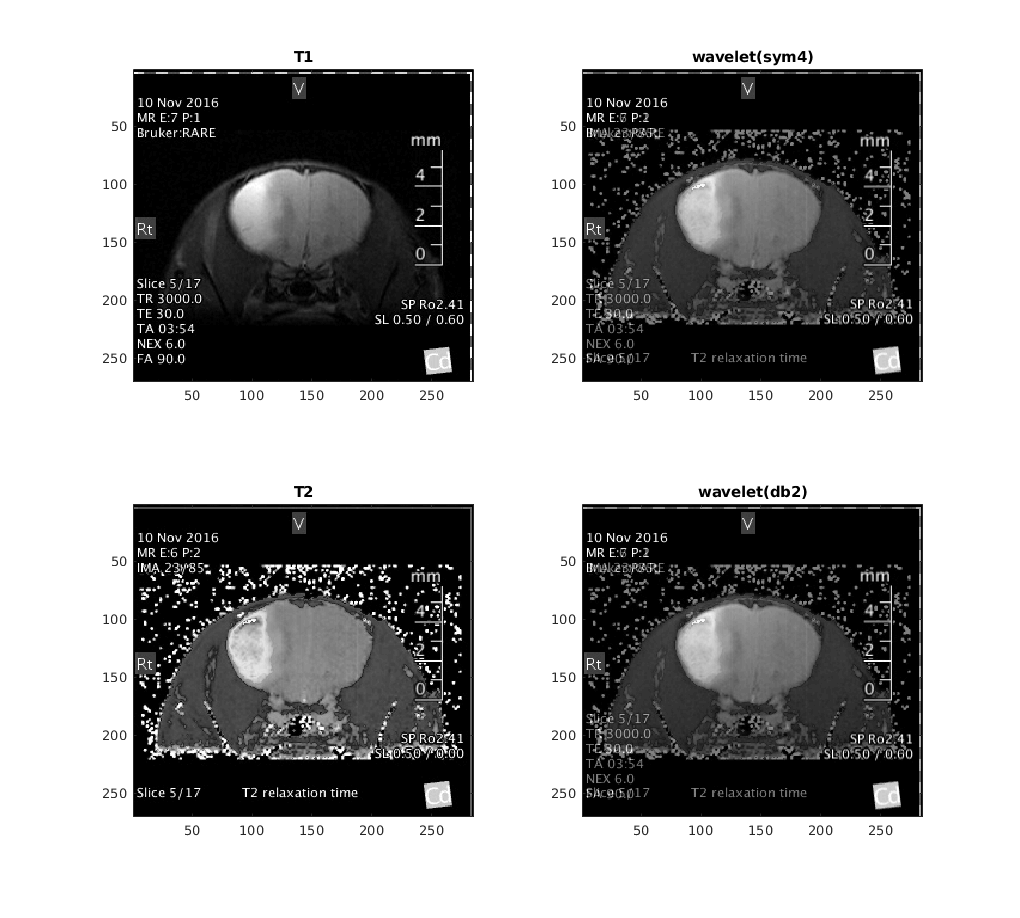
\includegraphics[width=0.7\textwidth]{waveletfusion}
	\caption{Slike stopljene koristeći dvije različite wavelet dekompozicije.}
	\label{fig:waveletfusion}
\end{figure}

\chapter{Usporedba rezultata}
Kao što se vidi na slici \ref{fig:waveletfusion}, metodom stapanja wavelet transformacijom dobivamo sliku koja izgleda kao prva T1 mapa snimke, ali su rubovi lezije oštriji i bolje vidljivi. 
Osim wavelet transformacije koristit ćemo i kvantizaciju Otsuovom metodom prije metode popunjavanja regije kako bi smanjili raspon sivih boja i dodatno povećali razliku u svjetlini na granicama lezije.
Otsuova metoda traži optimalnu podjelu razina sive na ograničeni broj tako da minimizira varijancu unutar razreda, a povećava varijancu između razreda. Koristimo ugrađenu MATLAB metodu $multithresh()$

\begin{figure}[H]
	\centering
	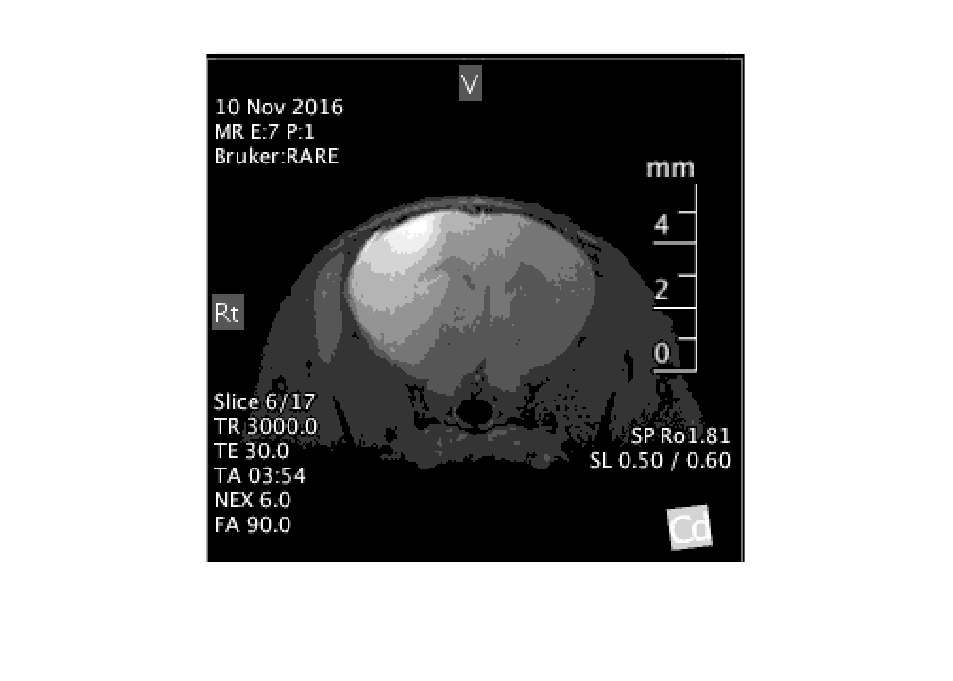
\includegraphics[width=0.7\textwidth]{thresh}
	\caption{Slika kvantizirana na 8 razina Otsuovom metodom}
	\label{fig:thresh}
\end{figure}

\begin{figure}[H]
	\centering
	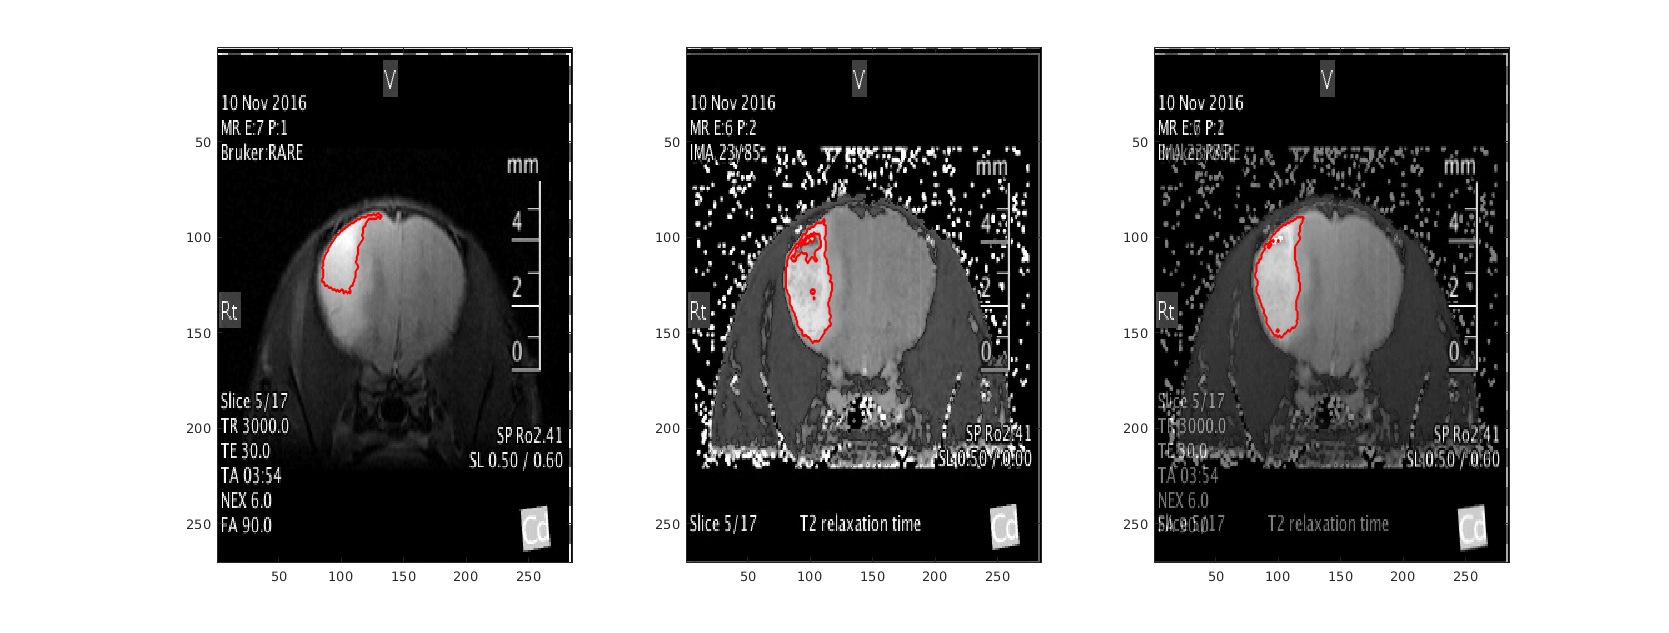
\includegraphics[width=0.9\textwidth]{results}
	\caption{Segmentirane lezije na odvojenim slikama i na slici kombiniranoj metodom wavelet transformacije}
	\label{fig:results}
\end{figure}

\section{Mjerenja lezije}
Veličinu lezije određujemo kao površinu presjeka, odnosno broj piksela unutar regije. Na rezultatima se vidi kako za T1 mapu skoro nikad ne dobivamo cijelu leziju, kod T2 ima manje odstupanja, a kod stopljene slike ???

% \begin{tabular}{l*{10}{c}}
% 	T1 & 1. & 2. & 3. & 4. & 5. & 6. & 7. & 8. & 9. & 10. \\
% 	\hline
% 	1. & 859 & 859 & 859 & 859 & 859 & 859 & 859 & 859 & 859 & 859 \\
% 	2. & 826 & 826 & 826 & 826 & 826 & 826 & 826 & 826 & 826 & 826 \\
% 	3. & 598 & 598 & 1064 & 1064 & 598 & 1064 & 1064 & 598 & 1064 & 598 \\
% 	4. & 992 & 863 & 863 & 863 & 863 & 863 & 863 & 992 & 863 & 863 \\
% 	5. & 646 & 1696 & 646 & 1696 & 646 & 646 & 646 & 1696 & 646 & 1696 \\
% 	6. & 3656 & 737 & 3656 & 737 & 737 & 737 & 3656 & 737 & 737 & 737 \\
% 	7. & 796 & 796 & 796 & 796 & 796 & 796 & 796 & 3957 & 796 & 796 \\
% 	8. & 834 & 3343	& 834 & 834 & 834 & 834 & 3343 & 834 & 834 & 834 \\
% 	\hline
% 	mean & 1150.9 & 1214.7 & 1193 & 959.4 & 769.9 & 828.1 & 1506.6 & 1312.4 & 828.1 & 901.1 \\
% 	std & 1019.7 & 921.7 & 1001.7 & 312.3 & 100.4 & 119.7 & 1238.1 & 1118.4 & 119.7 & 332.8
% 
% \end{tabular}

\begin{figure}[H]
	\centering
	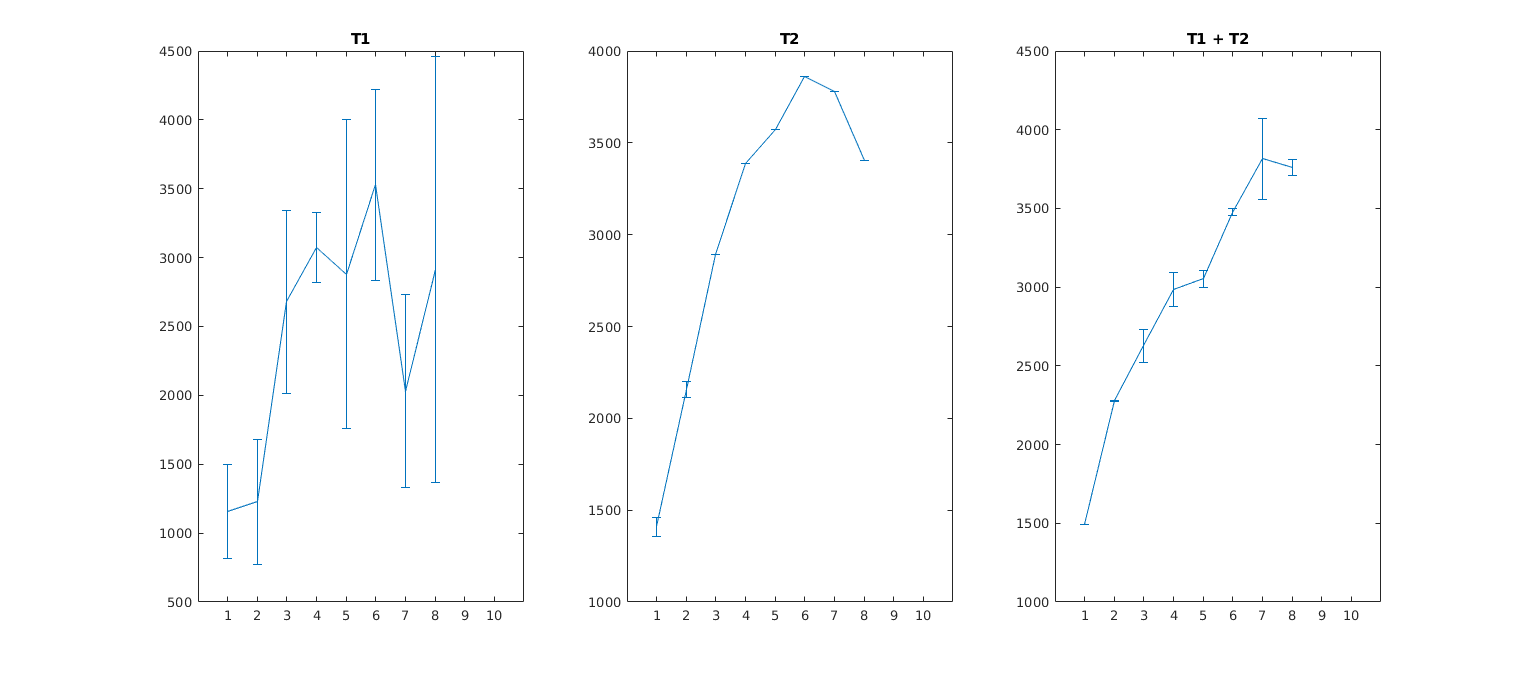
\includegraphics[width=0.9\textwidth]{error}
	\caption{Srednja površina lezije i standardna devijacija za svaki presjek u T1, T2 mapi i njihovoj kombinaciji.}
	\label{fig:error}
\end{figure}

\begin{figure}[H]
	\centering
	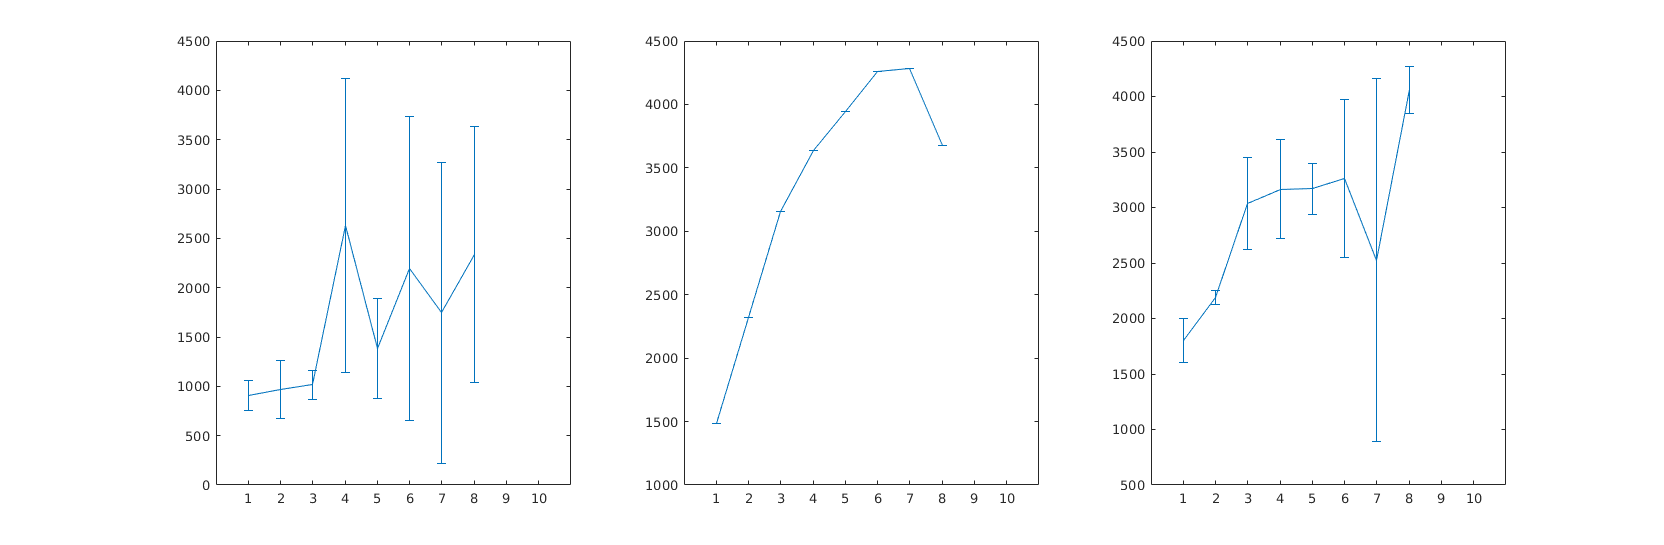
\includegraphics[width=0.9\textwidth]{errorQuant}
	\caption{Srednja površina lezije i standardna devijacija za svaki presjek u T1, T2 mapi i njihovoj kombinaciji sa kvantizacijom prije provođenja segmentacije.}
	\label{fig:errorQuant}
\end{figure}



\chapter{Zaključak}
Medicinske radiološke snimke ne daju uvijek u potpunosti jasnu sliku ciljanog objekta, odnosno abnornalnosti ili lezije. Kombiniranjem višesenzorskih snimaka možemo dobiti puno više informacija, poboljšati i dobiti jasniju sliku iz koje je lakše izvući bolje rezultate.

Kao izvorne slike dobivene su po dvije snimke istog presjeka, ali korištenjem različitih senzora. Prva slika ima visoku razlučivost i jasno razlikuje meko i tvrdo tkivo, ali se ne vide jasne granice lezije. Kod druge slike se jako dobro vide granice lezije, ali je razlučivost slabija. Kombiniranjem dviju slika dobivamo korisne informacije od obje slike. 

Kao dobra metoda stapanja slika se pokazala wavelet transformacija, ali i jednostavnije metode poput stapanja pomoću PCA. 

\bibliography{literatura}
\bibliographystyle{fer}

\begin{sazetak}
	Segmentacija slika je široko područje sa različitim rješenjima ovisnima o problemu. U medicinskim MRI snimkama dobivamo više informacija za svaki snimljeni sloj. U ovom radu ću istražiti metode preklapanja više mapa za svaki sloj MRI snimke, i metode segmentacije za određivanje površine lezija i odrediti preciznost postupka uz izračun greške i standardne devijacije.

	\kljucnerijeci{segmentacija, medicinske snimke, preklapanje slika}
\end{sazetak}

\engtitle{Automated image segmentation of lesions in MRI scans}
\begin{abstract}
	Image segmentation is a broad area of research with many different solutions dependant on the nature of the problem. In medical MRI imaging we get more information for each recorded slice. In this paper I will examine methods for image fusion of different maps of MRI images, and methods of segmentation for determining the area of lesions and determine the accuracy of these methods on the basis of error and standard deviation.

	\keywords{image segmentation, medical imaging, image fusion}
\end{abstract}
\end{document}
